The greatest eclipse is defined as the instant when the axis of the Moon's shadow cone gets closest to the centre of the Earth in a solar eclipse. This problem explores the geometry of this phenomenon, using the solar eclipse of $\text{29}^{\text{th}}$ May 1919 as an example, as it has great historical significance for being the first time astronomers were able to observationally verify general relativity. One of the scientific expeditions to observe this eclipse took place in the Brazilian city of Sobral.

The two following tables show the Cartesian and spherical coordinates of the Sun and the Moon at the time of the greatest eclipse. The system used for these coordinates is right-handed and has the origin at the centre of the Earth, the positive $x$-axis pointing towards the Greenwich meridian, and the positive $z$-axis pointing towards the North Pole. For the rest of this problem, this will be referred to as \textbf{system I}.

Spherical coordinates:

\begin{center}
    \begin{tabular}{|| c | c | c ||} 
         \hline
          & Centre of the Sun & Centre of the Moon\\ [0.5ex] 
         \hline\hline
         Radial Distance ($r$) & \SI{1.516e11}{\metre} & \SI{3.589e8}{\metre} \\ 
         \hline
         Polar Angle ($\theta$) & \ang{68;29;44.1} & \ang{68;47;41.6}\\
         \hline
         Azimuthal Angle ($\varphi$) & $-1^h 11^m 28.2^s$ & $-1^h 11^m 22.9^s$\\
         \hline
    \end{tabular}
\end{center}

Cartesian coordinates:

\begin{center}
    \begin{tabular}{|| c | c | c ||} 
         \hline
          & Centre of the Sun & Centre of the Moon\\ [0.5ex] 
         \hline\hline
         $x$ & \SI{1.342e11}{\metre} & \SI{3.185e8}{\metre}\\ 
         \hline
         $y$ & \SI{-4.327e10}{\metre} & \SI{-1.025e8}{\metre} \\
         \hline
         $z$ & \SI{5.557e10}{\metre} & \SI{1.298e8}{\metre} \\
         \hline
    \end{tabular}
\end{center}

For this problem, assume that the Earth is a perfect sphere.

\bigskip

\textbf{Note:} The spherical coordinates of a point $P$ are defined as follows:

\begin{itemize}
    \item Radial distance ($r$): distance between the origin ($O$) and $P$ (range: $r\geq 0$).

    \item Polar angle ($\theta$): angle between the positive $z$-axis and the line segment $OP$ (range: $\ang{0}\leq\theta\leq \ang{180}$).

    \item Azimuthal angle ($\varphi$): angle between the positive $x$-axis and the projection of the line segment $OP$ onto the $xy$-plane (range: $-12^h \leq \varphi < 12^h$).
\end{itemize}

\begin{figure}[H]
    \centering
    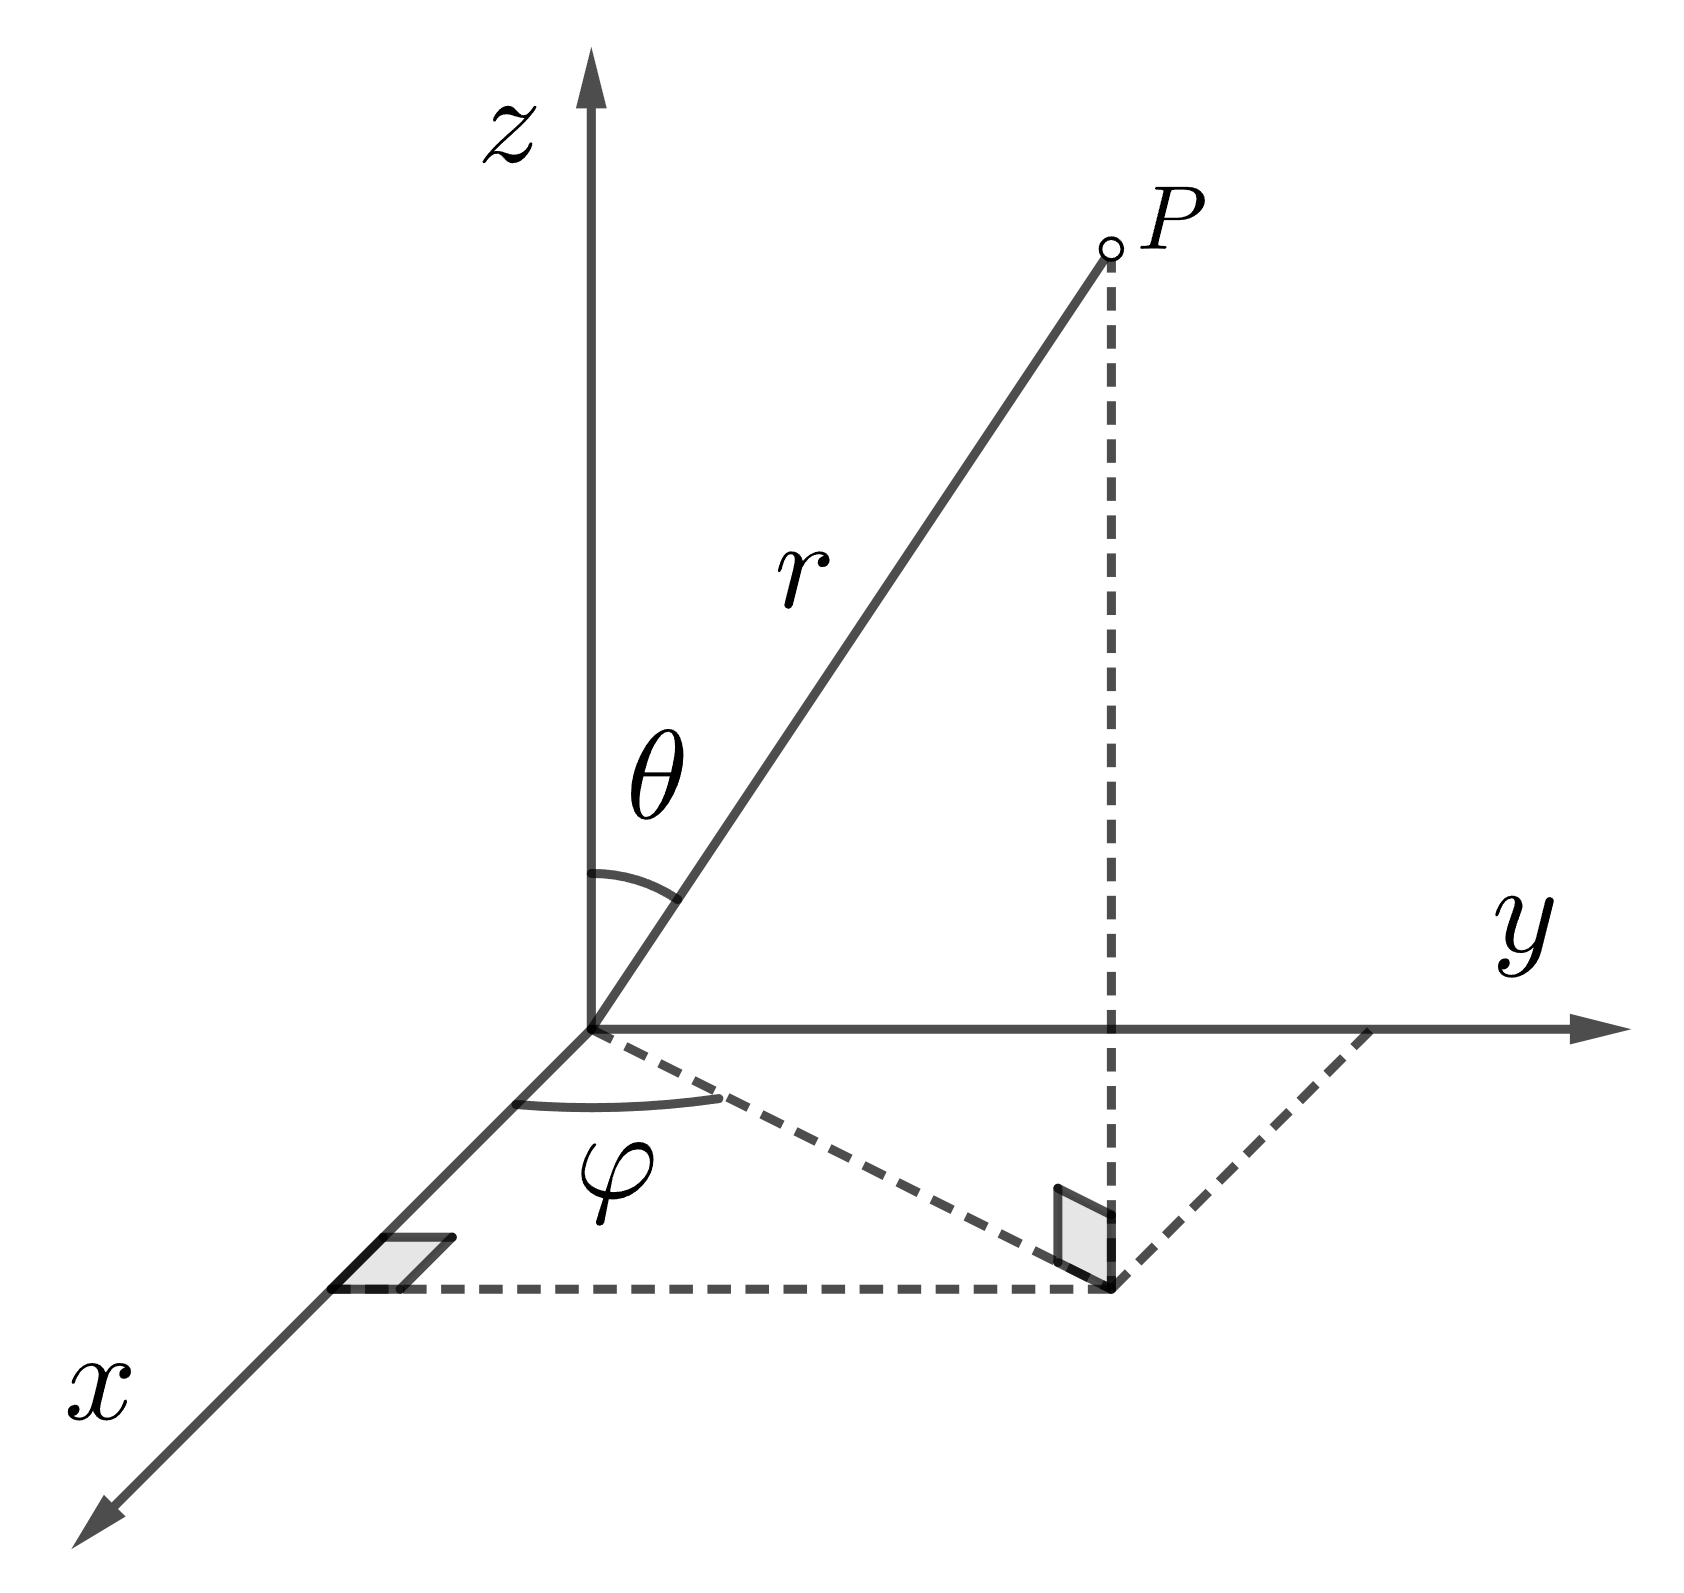
\includegraphics[width=0.6\textwidth]{2024/Theory/Figures/2024_TH_Q10_F1.png}
\end{figure}

\textbf{Part I: Geographic Coordinates (25 points)}

\begin{parts}
    \part[3] Determine the declination of the Sun and the Moon during the greatest eclipse for a geocentric observer.
    
    \part[3] Determine the right ascension of the Sun and the Moon at the time of the greatest eclipse for a geocentric observer. The local sidereal time at Greenwich at {that same moment} was $5^h 32^m 35.5^s$.
    
    \part[4] Find a unit vector that indicates the direction of the axis of the Moon’s shadow cone. This vector should point from the Moon to the vicinity of the centre of the Earth.
    
    \part[15] Determine the latitude and the longitude of the point where the axis of the Moon's shadow cone crosses the surface of the Earth during the greatest eclipse.
    
    \uplevel{\textbf{Part II: Duration of the Totality (50 points)}

    Precisely determining the duration of totality of a solar eclipse involves complex calculations that would be beyond the scope of this problem. However, it is possible to obtain a reasonable approximation for this value using the two following assumptions:
    
    \begin{itemize}
        \item The size of the umbra on the surface of the Earth remains roughly constant throughout totality at a given location.
        \item The velocity of the umbra on the surface of the Earth remains roughly constant throughout totality at a given location.
    \end{itemize}
    }    
    \part[10] Estimate the radius of the umbra during the greatest eclipse. In order to simplify the calculations, assume that the umbra is small enough that it can be considered approximately flat and that the axis of the Moon's shadow cone is extremely close to the centre of the Earth during the greatest eclipse.

    \part[3] Calculate the velocity of the Earth's rotation at the latitude of the centre of the umbra.
    
    \part[4] Determine the orbital velocity of the Moon at the instant of the greatest eclipse. Neglect the changes in the semi-major axis of the Moon’s orbit.

\uplevel{For the remaining items of this problem, assume that the tangential velocity of the Moon is roughly the same as the orbital velocity and neglect its radial component.}

In order to calculate the velocity of the umbra, it is convenient to define two new additional right-handed coordinate systems. \textbf{System II} is defined as follows:
\begin{itemize}
   \item Origin ($O_{\mathrm{II}}$): position of the Moon {at the instant of the greatest eclipse.}
   \item Positive $x$-axis: Tangent to the {declination circle}. Points eastwards.
   \item Positive $y$-axis: Tangent to the meridian of right ascension. Points northwards.
\end{itemize}

{\textbf{System III} is defined as follows:}

\begin{itemize}
   \item {Origin ($O_{\mathrm{III}}$): centre of the umbra {at the instant of the greatest eclipse.}}
   \item {Positive $x$-axis: Tangent to the {latitude circle}. Points eastwards.}
   \item {Positive $y$-axis: Tangent to the meridian of longitude. Points northwards.}
\end{itemize}

Note that {in both systems,} the $xy$-plane {is} tangent to the celestial sphere at the position of the {origin}.

System III is {similar} to system II, with the only difference being that the origin ($O_{\mathrm{III}}$) is at the centre of the umbra at the moment of the greatest eclipse.

    \part[14] Using System II, determine the velocity vector of the Moon during the greatest eclipse. Note that the intersection between the Celestial Equator and the lunar orbit that is closer to the position of the eclipse has a right ascension of $23^h 07^m 59.2^s$.

    \part[10]  Write the velocity vector of the Moon in System III. Note that in System I, the azimuthal angle difference between the positions of the origins $O_{\mathrm{II}}$ and $O_{\mathrm{III}}$ is negligible, so you should only take into account the difference in the polar angles.

    \part[6] Calculate the speed of the centre of the umbra along the surface of the Earth at the instant of the greatest eclipse.

    \part[3] Estimate the duration of the totality of the eclipse at the location with the coordinates found in part (d).

    \end{parts} 